\clearpage
\section{Installation Aktor}\label{sec:Aktor}
Das Aktor-Bord ist die physikalische Schnittstelle zu den Elektronischen Geräten. Die Relais K1 bis K4 können 250 Volt AC und 10 Ampere schalten. An den 0-10 Volt Ausgängen darf einen maximalen Strom von 4 mA bezogen werden.
\subsection{Anleitung einrichten}
\begin{figure}[H]
	\centering
	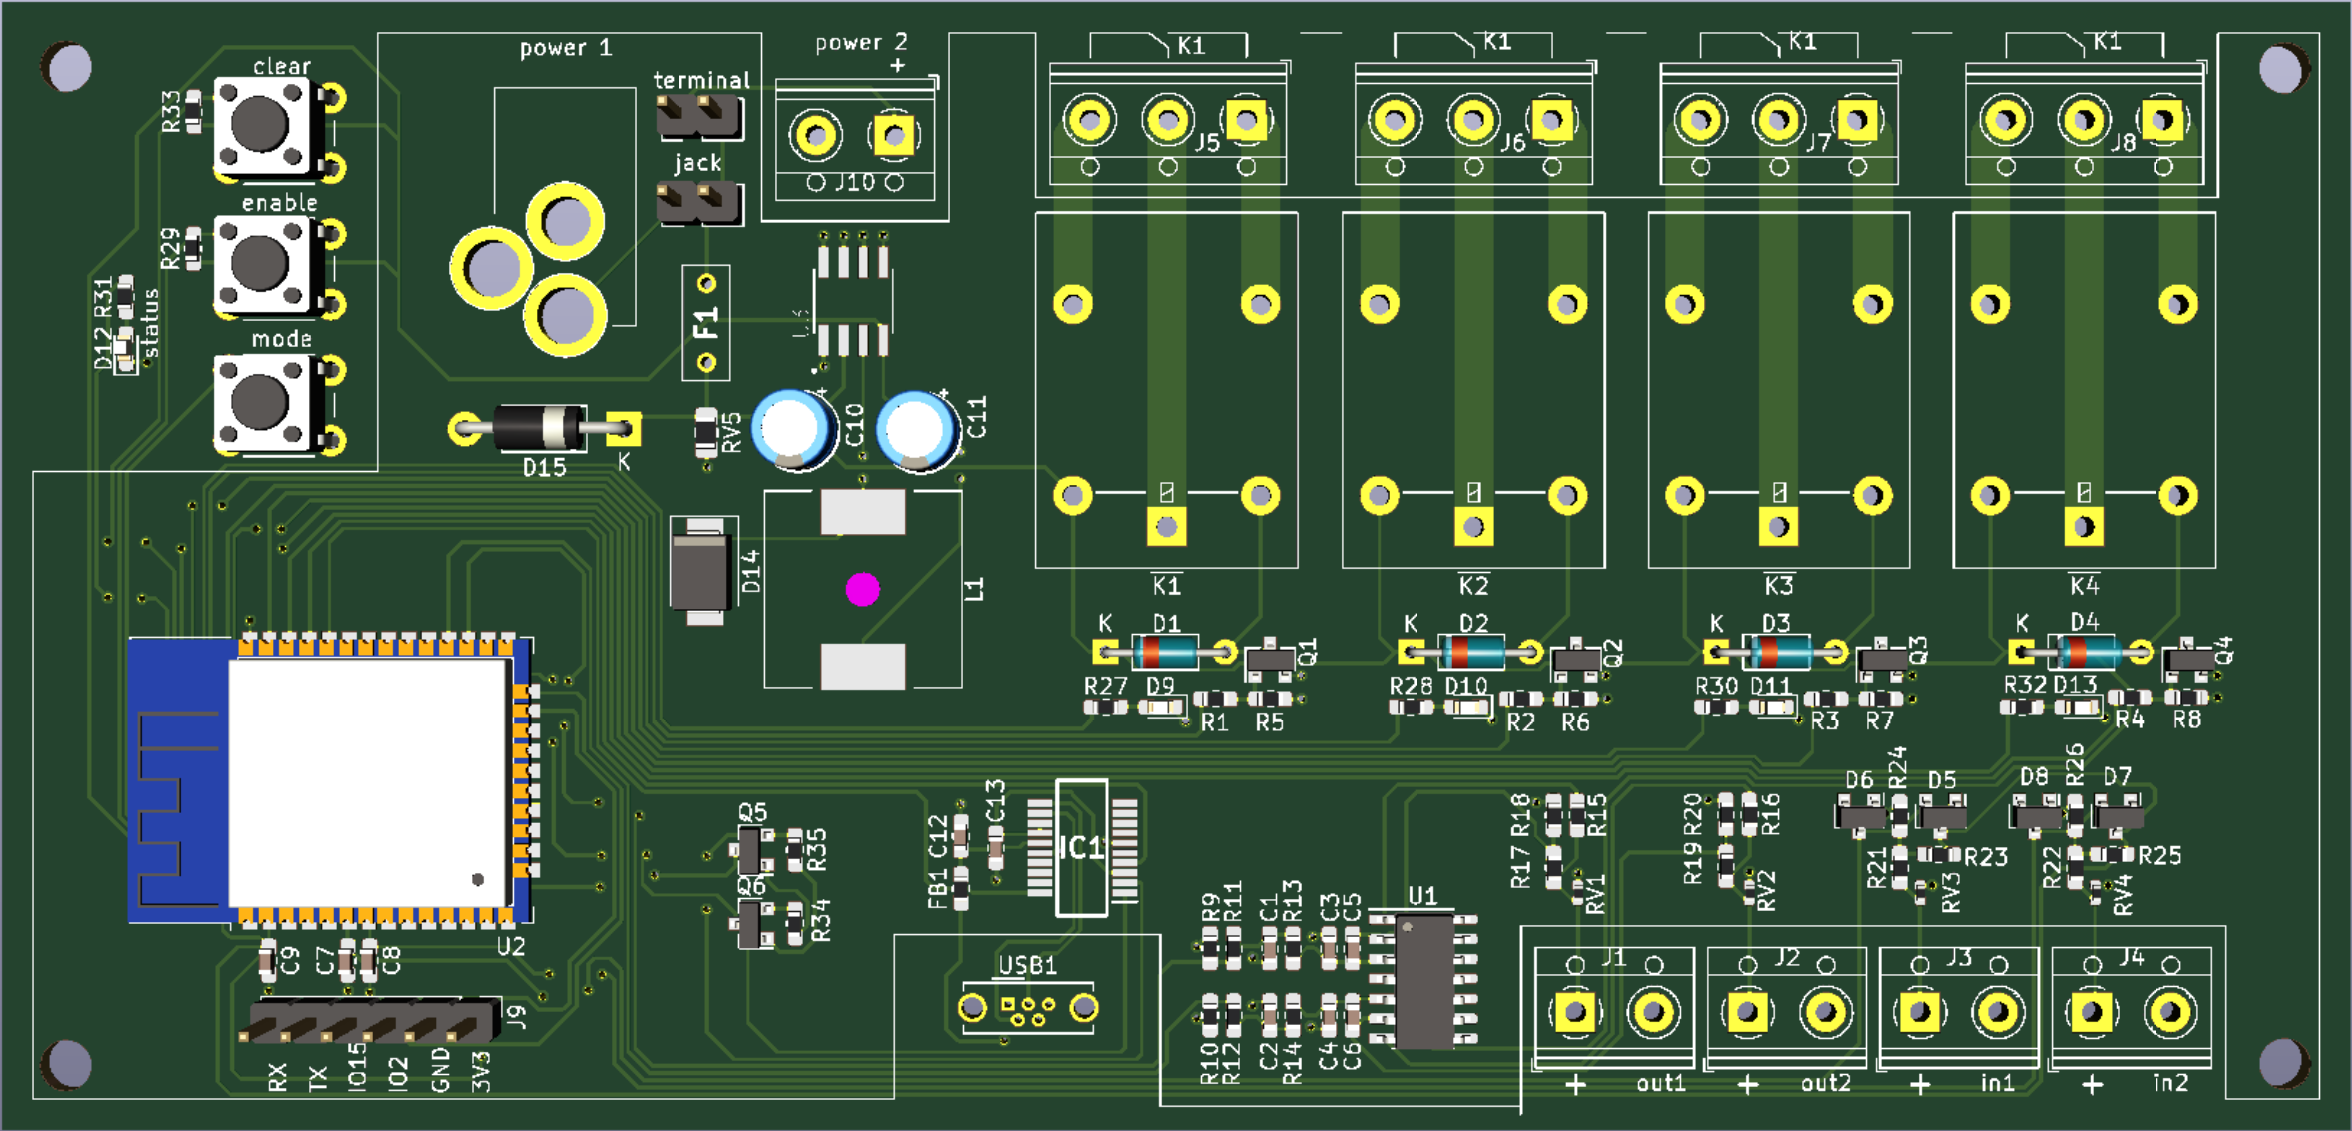
\includegraphics[width=\textwidth]{graphics/Aktorbaustein.png}
	\caption{Aktor Bord} 	
	\label{pic: OSGILayers}
\end{figure} 

\begin{enumerate}
	\item Das Gehäuse des Aktor-Bords, soll in eine Haupt- oder Unterverteilung eingebaut werden, wichtig ist zu beachten, dass sich dieser Standort innerhalb der eigenen WLAN-Reichweite befindet. Der Einbau ist im spannungslosen Zustand durchzuführen. \\
	\\
	\item Verbraucher wie Leuchten, Beschattungs-Systeme oder Ventilationen können in Schliesser- oder Öffnerbetrieb an den Relais K1 bis K4 angeschlossen werden. Wichtig ist zu beachten, dass die maximale Spannung von 250 Volt AC und maximaler Strom von 10 Ampere nicht überschritten wird.\\
		\\
	\item An den out1 und out2 Klemmen können Geräte mit einer 0-10 Volt Schnittstelle angeschlossen werden. Ein maximaler Strom von 4 mA darf nicht überschritten werden, damit die Spannung stabil bleibt.\\
	\\
	\item An den In1 und In2 Klemmen können 0-10 Volt Sensoren angeschlossen werden.\\
	\\
	\item Als Energieversorgung kann an den Power Klemmen eine 24 V DC Quelle angeschlossen werden. Das Board kann auch mit einem 24\,VDC Hohlstecker verbunden werden. Der Jumper muss entsprechend gesteckt werden, 'jack' für Hohlstecker oder "terminal" wenn die Speisung über Klemmen erfolgt. 
\end{enumerate}

\subsection{Inbetriebnahme}
Sobald das Aktor-Bord mit Spannung versorgt wird, startet der Mikrocontroller ein Access-Point und das Config-Portal des Bords. Mit einem beliebigen Gerät, kann nach einem WLAN-Netzwerk gesucht werden. Das Netzwerk hat den Namen 'Aktor' gefolgt von der 10 Stelligen Chip-ID des Mikrocontrollers. 
 
\begin{figure}[H]
	\begin{center}
	\begin{minipage}[b]{.3\linewidth} % [b] => Ausrichtung an \caption
		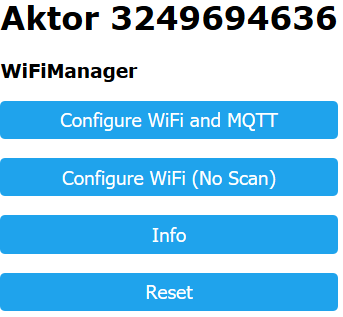
\includegraphics[width=\textwidth]{graphics/Configportal.PNG}
		\caption{Ansicht Configportal Frontseite}
	\end{minipage}
	\hspace{.1\linewidth}% Abstand zwischen Bilder
	\begin{minipage}[b]{.3\linewidth} % [b] => Ausrichtung an \caption
		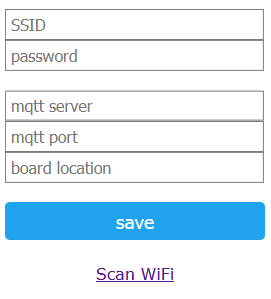
\includegraphics[width=\textwidth]{graphics/Configportal2.PNG}
		\caption{Parameter Config}
	\end{minipage}
\end{center}
\end{figure}
Mit der Funktion 'Scan WiFi' werden vorhanden Netzwerke angezeigt. Wird ein eigener MQTT Server installiert, kann an dieser Stelle die IP-Adresse angegeben werden, ansonsten der URL des öffentlichen MQTT-Broker. Der Port ist Default '1883' anzugeben. Die Eingabe bei 'board location' wird verwendet um MQTT-Topics zu generieren, sie muss also eindeutig sein und sollte keine Sonderzeichen beinhalten. Werden mehrere Aktor-Boards verbaut, unterscheiden sie sich an der 'bord location'. Mit der Taste 'save' werden die Eingaben gesichert und müssen bei einem erneuten Start nicht mehr eingegeben werden. Kann sich das Aktor Bord erfolgreich ins Lokale Netzwerk anmelden, blinkt die Status LED in einem regelmässigen Zyklus. Bei jeder Zustandsänderung der Statusleuchte wird eine Messung an den Eingängen In1 und In2 durchgeführt. 

\subsection{Programmierung}
Verschiedene Eigenschaften können mit dem Entwicklertool zusätzlich verändert werden, wenn der Programmcode des Mikrocontrollers bearbeitet wird. In der nachfolgenden Tabelle sind Default-Konfigurationen enthalten.
\begin{table}[H]
\centering
\begin{tabular}{|l|l|l|}
	\hline 
	Bezeichnung & Variable & Wert \\ 
	\hline 
	Zeit Interwall Messungen & NUM\_SEC & 10 \\ 
	\hline 
	Allgemeiner MQTT-Topic  & MQTT\_SERIAL\_PUB & 'data/aktorboard/' \\ 
	\hline 
	Messungen für Mean Wert ADC & I & 100 \\ 
	\hline  
\end{tabular} 	
\end{table}
Werden schnelle Reaktionszeiten vom System verlangt, von Befehlseingabe bis zur Ausführung, können Funktionen direkt im Programmcode eingebunden werden. So kann eine Reaktionszeit von 300\,ms erreicht werden. In diesem Fall wird in der Funktion 'callback()' definiert, wenn topic 'data/sensorboard/location/s1' empfangen wird, wird Relais1 schalten.
\subsection{Netzwerkeinstellungen ändern}
Soll sich das Aktor-Board in ein anderes Netzwerk anmelden, gibt es zwei verschiedene Möglichkeiten die Einstellungen zu ändern. Falls während des Startvorgangs die 'Mode' Taste betätigt wird, öffnet der Mikrocontroller das Config-Portal. Das Config-Portal wird ebenfalls geöffnet, wenn das einst eingetragene Netzwerk nicht mehr gefunden wird und keine Verbindung hergestellt werden kann.
\subsection{System Tasten}
Mit der Taste 'enable' wird manuell ein Neustart durchgeführt. \\
Mit der Taste 'mode' wird das Config-Portal eröffnet die Taste muss beim Startvorgang mindestens 5\,s Betätigt werden.\\
Die Taste 'clear' hat auf dem Prototyp Aktor-Board keine Funktion.

\subsection{Topics}
In der Nachfolgenden Tabelle sind die automatisch generierten Topics, welche weiter in Openhab verwendet werden, um festzulegen welches Relais bei welchem Befehl schaltet. Als 'location' wurde im Config-Portal in diesem Fall 'location' eingetragen.
\begin{table}[H]
	\centering
	\begin{tabular}{|l|l|}
		\hline 
		 Topic  & Funktion  \\ 
		\hline 
		data/aktorboard/location/K1 & Schaltet Relais 1  \\ 
		\hline
		data/aktorboard/location/K2 & Schaltet Relais 2  \\ 
		\hline
		data/aktorboard/location/K3 & Schaltet Relais 3  \\ 
		\hline
		data/aktorboard/location/K4 & Schaltet Relais 4  \\ 
		\hline 
		data/aktorboard/location/A1 & Schaltet 0-10V Output 1  \\ 
		\hline
		data/aktorboard/location/A2 & Schaltet 0-10V Output 2  \\ 
		\hline
		data/aktorboard/location/E1 & Publish 0-10V Input 1  \\ 
		\hline
		data/aktorboard/location/E2 & Publish 0-10V Input 2  \\ 
		\hline
	\end{tabular} 	
\caption{Generierte MQTT-Topics Aktor-Bord}
\label{tab: MQTT-Topics Aktor}
\end{table}
 
Mit den Topics werden die verschiedenen Anwendungen unterschieden, wobei sich der Zustand mit der Payload unterscheidet. Bei den Relais wird zwischen 'ON' und 'OFF' unterschieden. Bei den 0-10 Volt Inputs so wie Outputs enthält die Payload den entsprechenden Wert. 
